\section*{Abstract\raisebox{.3\baselineskip}{\normalsize\footnotemark}}
\footnotetext{\url{https://github.com/dedis/cothority/wiki}}

\paragraph{}
The Cothority\footnote{\url{https://github.com/dedis/cothority}} framework has been developed and maintained by the DeDiS laboratory at EPFL. This project provides a framework for developing, analysing, and deploying decentralised and distributed cryptographic protocols. A set of servers that runs these protocols and communicates among each other is referred to as a collective authority, or cothority, and the individual servers are called cothority servers or conodes. A cothority that executes decentralised protocols could be used for collective signing, threshold signing, or the generation of public-randomness, to name only a few options. The highest level of abstraction can be created by protocols like the collective signature (CoSi) protocol, the random numbers (RandHound) protocol, or the communication (Messaging) protocol used by the conodes to exchange data. Then come the services, which rely on these protocols. As of this writing, there exist several services: the Status service to enquire into the status of a conode, the CoSi service for collective signing, the Guard service that allows for the distributed encryption and decryption of passwords, the SkipChain service for storing arbitrary data on a permissioned blockchain, and the Identity service for distributed key/value pair storage. Applications (also called “apps”) run on top of these services, including Status, CoSi, Guard, collective identity skipchains (CISC), and proof-of-personhood (PoP). In this project report, we only concentrate on the last two, CISC and PoP.

\begin{figure}[h]
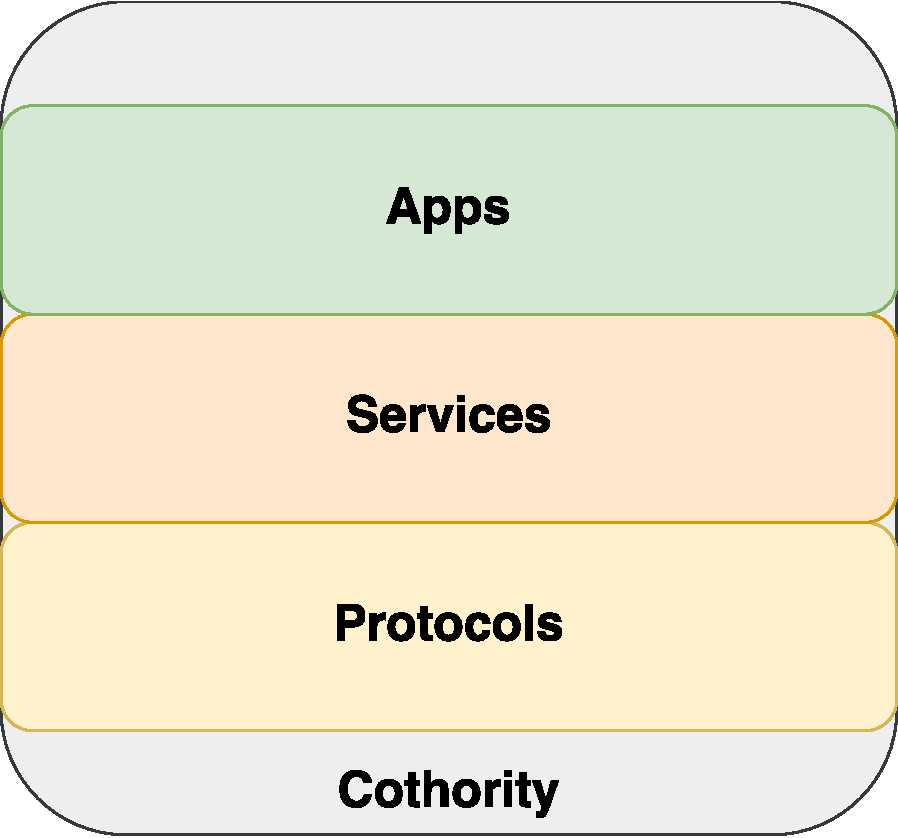
\includegraphics[scale=.5]{graphic/cothority.pdf}
\centering
\caption*{Cothority Framework}
\end{figure}

\subsubsection*{CISC App}

// TODO: INSERT

\subsubsection*{PoP App\raisebox{.3\baselineskip}{\normalsize\footnotemark}}
\footnotetext{\url{https://github.com/dedis/cothority/wiki/PoP}}

\paragraph{}
Anonymity on the internet is often a trade-off with accountability. Users want to be as anonymous as possible without losing rights and opportunities. This desire is in contrast with the needs of many online service providers who require this accountability to be able to provide users with a secure and high-quality experience. Captcha is one of the most frequently used methods to block non-human beings from accessing information. However, on one side, programs have become better and better at solving the Captcha queries, and on the other side, even human beings are occasionally unable to correctly decode a Captcha. The PoP app tries to remedy to this problem by providing so-called PoP Tokens, which can be considered to be a one-time captcha. These tokens are comparable to completely anonymous ID cards. The PoP Token proves that its holder is a human being who visited a specified place at a specified time, though it does so without revealing to which specific person the token refers.
